\section{Our Approach}
%\label{sec:approach}

\xj{introduce the new representation first.}
\xj{Add a new figure to explain the representation here. Show different room types and our representation. Add a paragraph here.}
%
Given multiple overlapping images of an indoor scene from different views, our approach produces the combined room layout represented by several room corners, as shown in Fig. \ref{fig:partial1}. 
%\xj{Explain more details of this new representation: add a figure. and more constraints? say, there are at most four points on each image? Split them to upper/lower parts?}
Under the Manhattan world assumption \cite{coughlan1999manhattan}, a 3D room can be typically modeled as a cube that can be represented by eight corners.
The room layout in a single view is the projection of the cube, while only part of it can be visible. 
Intuitively, there should be 0 to 4 room corners visible in a single-view image. 
%
%In this section, we are going to recover the room layout for perspective images from different views. 
Previous DNN-based techniques of room layout estimation typically represent the room layout as a segmentation of semantic surfaces including walls, ceilings and floors~\cite{dasgupta2016delay, ours} or as the semantic boundaries or intersection points among them \cite{ren2016coarse}. 
%
These representations have proved valid and reasonable. 
However, due to the overlaps across views, they all carry too much redundant predictions and are inconvenient for combination under the circumstances of multi-view layout estimation. 
Out of this reason, we propose a more concise representation of a room layout using the corners only.
This representation avoids extra efforts on classifying the room layout topology, and can be easily used to integrating multiple views.
\xj{Why are the previous representation inconvenient? why ours are better? ours are also redundant in multiple views. }

%
%When the overall FOV of the multi-view images contains the entire room, we can recover the whole-room layout, better viewed in panorama, Fig. \ref{fig:results2}. 
%
\xj{then pipeline.}
Fig. \ref{fig:overview} shows the pipeline of our algorithm. 
First, we estimate the partial room layout separately in each image using an encoder-decoder structure, as described in Sec. \ref{sec:layout}. 
Then the estimated partial room layouts are integrated into a combined probability map, based on the geometric transformations between images. 
We use a linear blending to average the predictions from different views, and select the points of the maximum responses as the room corners, as described in Sec. \ref{sec:merging}. 

 

\begin{figure*}[ht]
	\centering
	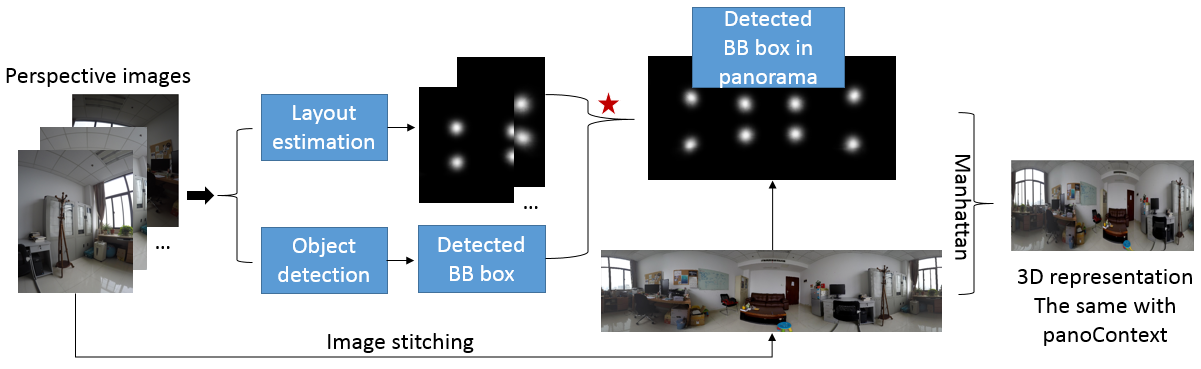
\includegraphics[width=\linewidth]{figs/ppline.png}
	\caption{Our pipeline consists of two main steps. First, the SVNet is applied to estimate the probability map for each image separately. Secondly, the input multi-view images are composed together according to the \xj{estimated or pre-calibrated?} transformations $f$. We use the same transformations $f$ to generate a combined probability map of the room corners. The final result is obtained by a simple post-processing \xj{no post-processing is shown in the fig.}. }
	\label{fig:overview}
\end{figure*}

\subsection{Single-view Layout Estimation}
\label{sec:layout}

%
%A direct way to achieve our goal is to utilize existing methods to estimate the layout for each view, and then combine these representations to produce the complete-room 3D layout. 
%However, this method is not efficient due to many redundant predictions caused by overlaps across views. 
\comments{
To avoid redundant predictions or even to benefit from them, we propose a \emph{secondary representation} of a room layout on perspective images. The room layout under each view is only represented by the intersections of vertical walls and ceiling or floor. We call these intersections secondary keypoints. 
\xj{What about the case when there in only one wall surface?}
Obviously, without the extra intersections of two semantic planes on the image boundaries, we cannot recover the room layout from a single perspective. However, these secondary keypoints in overlapping views are sufficient to reconstruct the 3D layout of the entire room. Compared to previous representations, our secondary keypoints are quite simplified and easier to train. It also naturally avoids a lot of redundant predictions. 
}

%\comments{ motivated by \cite{LeeRoomNet17} and the studies on human pose estimation \cite{tompson2014joint,pfister2015flowing}, we formulate the room corners on the image plane as 2D Gaussian centered at their locations. The standard deviation is set to 40 pixels in our case. \xj{this format is for training, right?}
%


%
Compared to previous representations, our corner-based representation is quite simplified and easier to train. 
It also naturally avoids a lot of redundant predictions. 
\xj{remove all "secondary representation".}

} 


 
Under our corner-based layout representation, we predict the corner positions for each view separately using a neural network. 
Considering the inherent semantic differences, we divide the room corners into two categories: the upper corners which are the intersection of two walls and ceiling, and the lower corners which are the intersection of two walls and floor. 
In consequence, the goal of our single-view net should be estimating the probability maps of these two types of room corners for the input image.

We adopt the encoder-decoder architecture proposed by \cite{LeeRoomNet17} with modifications, since it is an end-to-end framework without complex post-processing. 
%
Our layout estimation network for a single-view image, called SVNet, is shown in Fig.~\ref{fig:network}. 
%It is designed to estimate the room corners in a single-view image. 
%Our network for room corner estimation from a single-view image is shown in Fig.~\ref{fig:network}.
We mainly make two modifications on the decode part and classification branch. 
First, as our corner-based representation is more concise, we remove the recurrent structure in \cite{LeeRoomNet17} for efficiency, and we add more upsampling layers and convolution layers to upsample the feature maps from the bottleneck layer to get the same resolution with the input image as a compensation for accuracy. 
The final convolution layer is adapted to output a $w \times h \times 2$ probability array $T$ for our new representation, where $w$ and $h$ stand for the width and length of the input image. 
Each of the two slices can be viewed as a probability map for the upper corners and lower corners respectively. 
Secondly, \cite{LeeRoomNet17} delineates room layout using 2D keypoints. The semantic boundaries can be recovered by connecting the detected 2D keypoints in a specific order. As the connection order differs between room topologies, they have to add a classification branch in their network to classify the room type, and the final performance rely on the classification accuracy. 
Unfortunately, the accuracy is not satisfied. 
We naturally avoid this situation by using our representation. The simplified representation divides the room corners into only two categories and applies to all room types. 
Therefore, we remove the classification branch in our network architecture.
 
\begin{figure}
	\centering
	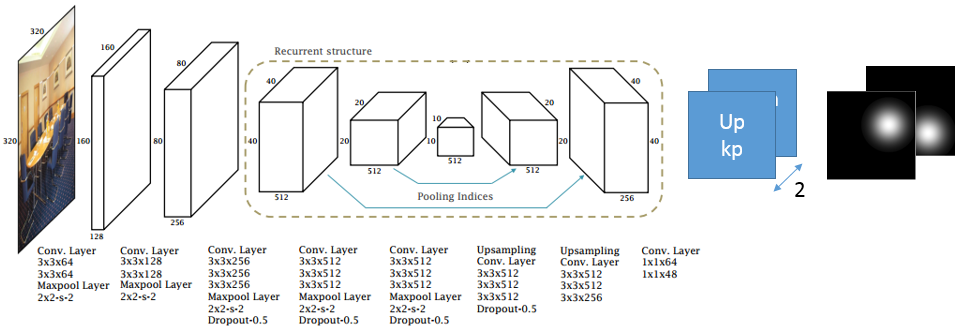
\includegraphics[width=\linewidth]{figs/network.png}
	\caption{Network architecture. The encoder part is topologically identical to the VGG16 network. It encodes the $320 \times 320$ input images to $10 \times 10$ feature maps. Then the decoder part upsample the feature maps from the bottleneck layer to full input resolution. }
	\label{fig:network}
\end{figure}

\noindent\textbf{Training.} 


While our method could take multiple images under different view directions of arbitrary field of view, we generate our training dataset using the PanoContext dataset \cite{zhang2014panocontext} and relabeled Stanford 2D-3D dataset \cite{layoutnet} to generate multi-view images for training. 
The PanoContext dataset contains 500 annotated panoramic images. We project these panorama into multiple $320 \times 320$ images at different views using the toolkit provided by \cite{zhang2014panocontext}. 
\xj{The number of views in the training? }

The ground truth locations of the room corners are obtained using the same transformations and are further transformed into the Gausian representation. 
While the output is a probability map, we produce the ground-truth map for each image by generating a 2D Gaussian centered at the location of each groundtruth corner with $\sigma=40$ pixels, similar with \cite{LeeRoomNet17,tompson2014joint,pfister2015flowing}.
%
Euclidean loss is used to regress the probability map of room corners. 
Because the background area is much larger than the corner areas in the probability maps, we adjust the distribution imbalance between foreground and background pixels by degrading the gradient weight of background pixels with a coefficient of 0.2.
\xj{Training parameters?}

%To obtain multiple overlapping perspective images, we project the panoramic images into different views using the toolkit provided by \cite{pano}. The ground truth of the secondary keypoints is represented by several 2D Gaussian heatmaps centered at their locations. We adjust the distribution imbalance between foreground and background pixels by degrading the gradient weight of background pixels with a coefficient of 0.2.

%The RoomNet-basic struture in \cite{RoomNet} is adopted in our training stage for efficiency. We first pretrain the Network on LSUN \cite{LSUN2016} training set. Then, to finetune the model on images from different views in the same room, we project the panorama from \cite{PanoContext} to $k$ views. We set $k$ to 12 and 24 in our experiment. The layout ground truth is relabeled using the same projection. 

%The secondary keypoints can be divided into two categories according to semantics: the intersection of two walls and ceiling or the intersection of two walls and floor.\xj{Move this sentence to the representation paragraph.}

%We train the network to regress these two kinds of keypoints separately in order to eliminate the ambiguity between them. For this reason, the output of our network is a $w \times h \times 2$ probability array $T$, where $w$ and $h$ stand for the width and length of the input image. Each of the 2 slices can be viewed as a probability map for the secondary keypoints in a corresponding category. 


\subsection{Layout Composition}
\label{sec:merging}
After we predict the probability maps of the room corners for each image, we then composite them to generate a layout in a larger field of views. 
First, we align the input images under different views by estimating the transformation $f$ between image plane and the composition image plane. 
%First, the input multi-view images are projected into a combined image using the camera poses, we formulate this view transformations as a function $f$. 
Then, we sum over the third dimension \xj{why third dimension?} of the probability array $T$ for each image to get a heatmap $\hat{T}$ depicting all included room corners. 
Next, we use the same mapping function $f$ to map the heatmap $\hat{T}$ from different views into the composition image plane. 
A linear blending along horizontal lines \xj{why along horizontal lines?} is applied to average the predictions of the overlapping area between different views, as shown in Fig. \ref{fig:blending}. 
\xj{Explain the different between two subfigures. }

%
After that, we pick the points with the maximum responses as the room corners. 
At this stage, we first reduce the noise in $\hat{T}$ caused by unsatisfactory predictions from particular perspectives \xj{how to reduce the noise?}.
We calculate the LOG response of $\hat{T}$ at a certain scale (depending on the radius of the room corners), $\sigma$ is set to 21 in our case, and use the LOG response as our new heatmap.
%
Then, we follow the post-processing method in \cite{zou2018layoutnet} to obtain the locations of the room corners in the combined heatmap. In brief, the combined heatmap is summed across rows to find $m$ local maxima for columns, then $n$ largest peaks are found along each of the $m$ columns. In this way, we attain the locations of $m \times n$ room corners. In the case of panorama, $m$ is set to 4 and $n$ is set to 2. The whole room layout can be reconstructed by connecting these eight keypoints. 
\xj{Confusing and repeated ..with last paragraph.}



\begin{figure}
	\centering
	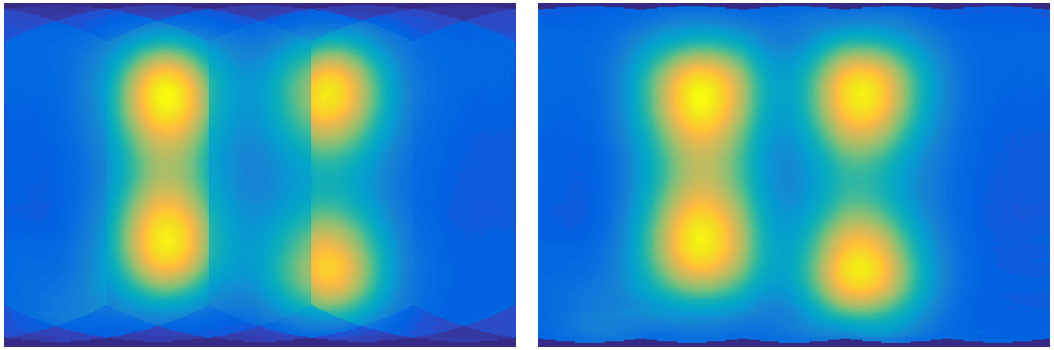
\includegraphics[width=\linewidth]{figs/blending.png}
	\caption{The combined probability map. Using simply average (left) or linear blending along horizontal lines (right).}
	\label{fig:blending}
\end{figure}


\comments{
\subsection{Alignment and 3D Reconstruction}
\label{sec:align}

(Optional and undone) In this section, we align the panoramic images to make sure that wall-wall boundaries are vertical to the floor. If we use the panorama to generate testing images, this step can be omitted as the reprojected panoramic images naturally met this alignment condition. Then the aligned panorama can be further rendered into a 3D representation. These two steps are implemented using existing techniques but the rendering part is not yet available. 
}
